\documentclass[a4paper,12pt]{extarticle}
\usepackage[utf8x]{inputenc}
\usepackage[T1,T2A]{fontenc}
\usepackage[russian]{babel}
\usepackage[hidelinks]{hyperref}
\usepackage{indentfirst}
\usepackage{listings}
\usepackage{color}
\usepackage{here}
\usepackage{array}
\usepackage{multirow}
\usepackage{graphicx}
\usepackage{subcaption} 
\usepackage{mathtools}
\usepackage{listings}

\usepackage{caption}
\renewcommand{\lstlistingname}{Программа} % заголовок листингов кода

\bibliographystyle{ugost2008ls}

\usepackage{listings}
\lstset{ %
extendedchars=\true,
keepspaces=true,
language=C,						% choose the language of the code
basicstyle=\footnotesize,		% the size of the fonts that are used for the code
numbers=left,					% where to put the line-numbers
numberstyle=\footnotesize,		% the size of the fonts that are used for the line-numbers
stepnumber=1,					% the step between two line-numbers. If it is 1 each line will be numbered
numbersep=5pt,					% how far the line-numbers are from the code
backgroundcolor=\color{white},	% choose the background color. You must add \usepackage{color}
showspaces=false				% show spaces adding particular underscores
showstringspaces=false,			% underline spaces within strings
showtabs=false,					% show tabs within strings adding particular underscores
frame=single,           		% adds a frame around the code
tabsize=2,						% sets default tabsize to 2 spaces
captionpos=t,					% sets the caption-position to top
breaklines=true,				% sets automatic line breaking
breakatwhitespace=false,		% sets if automatic breaks should only happen at whitespace
escapeinside={\%*}{*)},			% if you want to add a comment within your code
postbreak=\raisebox{0ex}[0ex][0ex]{\ensuremath{\color{red}\hookrightarrow\space}},
texcl=true,
inputpath=listings,                     % директория с листингами
}

\usepackage[left=2cm,right=2cm,
top=2cm,bottom=2cm,bindingoffset=0cm]{geometry}

%% Нумерация картинок по секциям
\usepackage{chngcntr}
\counterwithin{figure}{section}
\counterwithin{table}{section}

%%Точки нумерации заголовков
\usepackage{titlesec}
\titlelabel{\thetitle.\quad}
\usepackage[dotinlabels]{titletoc}

%% Оформления подписи рисунка
\addto\captionsrussian{\renewcommand{\figurename}{Рисунок}}
\captionsetup[figure]{labelsep = period}

%% Подпись таблицы
%\DeclareCaptionFormat{hfillstart}{\hfill#1#2#3\par}
%\captionsetup[table]{format=hfillstart,labelsep=newline,justification=centering,skip=-10pt,textfont=bf}

%% Путь к каталогу с рисунками
\graphicspath{{fig/}}

%% Внесение titlepage в учёт счётчика страниц
\makeatletter
\renewenvironment{titlepage} {
 \thispagestyle{empty}
}
\makeatother

\DeclarePairedDelimiter\abs{\lvert}{\rvert}%
\DeclarePairedDelimiter\norm{\lVert}{\rVert}%

\usepackage{amsmath}

\lstset{language=Java} 

\begin{document}	% начало документа

% Титульная страница
\begin{titlepage}	% начало титульной страницы

	\begin{center}		% выравнивание по центру

		\large Санкт-Петербургский политехнический университет Петра Великого\\
		\large Институт прикладной математики и механики \\
		\large Высшая школа прикладной математики и вычислительно физики \\[6cm]
		% название института, затем отступ 6см
		
		\huge Вычислительные комплексы\\[0.5cm] % название работы, затем отступ 0,5см
		\large \textbf{Курсовой проект}\\[5.1cm]

	\end{center}


	\begin{flushright} % выравнивание по правому краю
		\begin{minipage}{0.25\textwidth} % врезка в половину ширины текста
			\begin{flushleft} % выровнять её содержимое по левому краю

				\large\textbf{Работу выполнил:}\\
				\large Колесник Виктор\\
				\large {Группа:} 3630102/70201\\
				
				\large \textbf{Преподаватель:}\\
				\large к.ф.-м.н., доцент\\
				\large Баженов Александр Николаевич

			\end{flushleft}
		\end{minipage}
	\end{flushright}
	
	\vfill % заполнить всё доступное ниже пространство

	\begin{center}
	\large Санкт-Петербург\\
	\large \the\year % вывести дату
	\end{center} % закончить выравнивание по центру

\end{titlepage} % конец титульной страницы

\vfill % заполнить всё доступное ниже пространство


% Содержание
\renewcommand\contentsname{\centerline{Содержание}}
\tableofcontents
\newpage

\listoffigures
\newpage


\section{Постановка задачи}

Требуется решить ИСЛАУ с применением аппарата линейного программирования для проведения регуляризации рассматриваемой системы.

\subsection{Конкретизация задачи}
Дана ИСЛАУ с точечной матрицей $A$ и интервальной правой частью $\textbf{b}$: \\
\begin{equation}
	A =
	\begin{pmatrix}
		3 & 3 & 9 \\
		5 & 2 & 6 \\
		4 & 2 & 6
	\end{pmatrix}
\end{equation}
\begin{equation}
	\textbf{b} =
	\begin{pmatrix}
		[0, 1] \\
		[-2, 0] \\
		[4, 6]
	\end{pmatrix}
\end{equation}
С помощью распознающего функционала Tol($x$) можно убедиться, что у системы нет решений. Используя функцию tolsolvty были найдены максимум распознающего функционала и значение аргумента, в котором он достигался: \\
\begin{equation}
	\max \text{Tol} = -2
\end{equation}
\begin{equation}
	\arg \max \text{Tol}=
	\begin{pmatrix}
		7.3788 * 10^{-8} \\
		0.1 \\
		0.3
	\end{pmatrix}
\end{equation}
Так как $\max \text{Tol} < 0$, допусковое множество ИСЛАУ пусто.



\section{Решение}

\subsection{Регуляризация ИСЛАУ}
Проведем $l_1$-регуляризацию для получения решения. Изменим радиусы компонент вектора $\textbf{b}$ их поэлементным домножением на вектор масштабирующих множителей $w$: \\
\begin{equation}
	\textbf{b}=
	\begin{pmatrix}
		[\text{mid} b_1 - \text{rad} b_1; \text{mid} b_1 + \text{rad} b_1] \\
		[\text{mid} b_2 - \text{rad} b_2; \text{mid} b_2 + \text{rad} b_2] \\
		[\text{mid} b_3 - \text{rad} b_3; \text{mid} b_3 + \text{rad} b_3]
	\end{pmatrix} \rightarrow \tilde{\textbf{b}} = 
	\begin{pmatrix}
		[\text{mid} b_1 - w_1 \text{rad} b_1; \text{mid} b_1 + w_1 \text{rad} b_1] \\
		[\text{mid} b_2 - w_2 \text{rad} b_2; \text{mid} b_2 + w_2 \text{rad} b_2] \\
		[\text{mid} b_3 - w_3 \text{rad} b_3; \text{mid} b_3 + w_3 \text{rad} b_3]
	\end{pmatrix}
\end{equation}
При этом масштабирующие множители подбираются так, чтобы регуляризованная ИСЛАУ $A x=\textbf{b}$ стала разрешимой, а сумма этих множителей $\sum w_i$ была минимально возможной. \\

Накладывая на масштабирующие множители естественное требование их неотрицательности, и введя вектор $u = \begin{pmatrix}
	x \\
	w
\end{pmatrix}$, можно записать полученную задачу в виде:
\begin{equation}
	\begin{cases}
		c u = \begin{pmatrix}
			0 & 0 & 0 & 1 & 1 & 1
		\end{pmatrix} \begin{pmatrix}
		x_1 \\
		x_2 \\
		x_3 \\
		w_1 \\
		w_2 \\
		w_3
	\end{pmatrix} \rightarrow \min \\
	u_{4,5,6} \geq 0 \\
	C u \leq r, \text{ где } C = \begin{pmatrix}
		-A & -\text{diag} (\text{rad} \textbf{b}) \\
		A & -\text{diag} (\text{rad} \textbf{b})
	\end{pmatrix}, r = \begin{pmatrix}
		-\text{mid} \textbf{b} \\
		\text{mid} \textbf{b}
	\end{pmatrix}
	\end{cases}
\end{equation}
Полученная задача является задачей линейного программирования. В результате решения определяются одновременно необходимые масштабирующие множители и соответствующее им появившееся в результате регуляризации решение ИСЛАУ.

\subsection{Регуляризация заданной ИСЛАУ}
Для конкретной ИСЛАУ получим следующие вектор и матрицу для задачи линейного программирования:
\begin{equation}
	r=
	\begin{pmatrix}
		-0.5 \\
		-1 \\
		-5 \\
		0.5 \\
		1 \\
		5
	\end{pmatrix}
\end{equation}
\begin{equation}
	C =
	\begin{pmatrix}
		-3 & -3 & -9 & -0.5 & 0 & 0 \\
		-5 & -2 & -6 & 0 & -1 & 0 \\
		-4 & -2 & -6 & 0 & 0 & -1 \\
		3 & 3 & 9 & -0.5 & 0 & 0 \\
		5 & 2 & 6 & 0 & -1 & 0 \\
		4 & 2 & 6 & 0 & 0 & -1
	\end{pmatrix}
\end{equation}



\section{Результаты}
\subsection{Полученные результаты}
Воспользуемся двумя методами решения задач линейного программирования: simplex и interior-point. Получим следующие результаты:
\begin{itemize}
	\item Simplex-метод \\
		\begin{equation}
			x \approx
			\begin{pmatrix}
				-0.4444 \\
				0 \\
				0.2037
			\end{pmatrix}, w \approx \begin{pmatrix}
				0 \\
				0 \\
				5.5555
			\end{pmatrix}, \min c u = 5.5555
		\end{equation}
	
	\item Interior-point-метод \\
		\begin{equation}
			x \approx
			\begin{pmatrix}
				-0.4444 \\
				0.0608 \\
				0.1834
			\end{pmatrix}, w \approx \begin{pmatrix}
				0 \\
				0 \\
				5.5555
			\end{pmatrix}, \min c u = 5.5555
		\end{equation}
\end{itemize}
Из результатов видно, что первая координата имеет одинаковое значение при решении обоими методами. Кроме того, соответствующий масштабирующий множитель равен нулю. Проверим, что решения с $x_1=-0.4444$ оптимальны и устойчивы. Для этого зададим ограничение $x_1 \geq -0.4444 + 0.0001=-0.4443$. Получим следующие результаты:
\begin{itemize}
	\item Simplex-метод \\
	\begin{equation}
		x \approx
		\begin{pmatrix}
			-0.4443 \\
			0 \\
			0.2036
		\end{pmatrix}, w \approx \begin{pmatrix}
			0 \\
			0.0003 \\
			5.5555
		\end{pmatrix}, \min c u = 5.5556
	\end{equation}
	
	\item Interior-point-метод \\
	\begin{equation}
		x \approx
		\begin{pmatrix}
			-0.4443 \\
			0.0609 \\
			0.1833
		\end{pmatrix}, w \approx \begin{pmatrix}
			0 \\
			0.0003 \\
			5.5555
		\end{pmatrix}, \min c u = 5.5556
	\end{equation}
\end{itemize}
Значение суммы масштабирующих коэффициентов стало больше, чем соответствующее значение при решении задачи без ограничения на $x_1$. Значит, решения с $x_1=-0.4444$ являются оптимальными и устойчивыми.

\subsection{Ограничения на $x_2$}
Если позволить $x_1$ принимать значение $-0.4444$, то одинаково хорошие решения с точки зрения суммы масштабирующих коэффициентов можно получить при любых ограничениях на одну из координат $x_2$ или $x_3$. Попробуем ограничивать значение $x_2$ интервалами шириной 0.2: $x_2 = [x_{2 \min}; x_{2 \min} + 0.2]$. Посмотрим на зависимость других координат решения, соответствующего масштабирующего коэффициента и целевой функции от выбора ограничения на $x_2$. Результаты представлены на графиках для 2 методов решения задачи ЛП. \\
\begin{figure}[h]
	\centering
	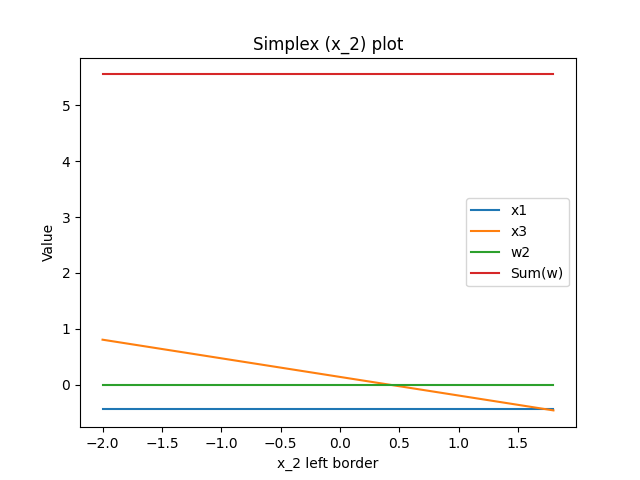
\includegraphics[width=0.5\textwidth]{simplex(x_2).png}
	\caption{Зависимость от ограничений на $x_2$ при решении Simplex-методом}
\end{figure}
\begin{figure}[h]
	\centering
	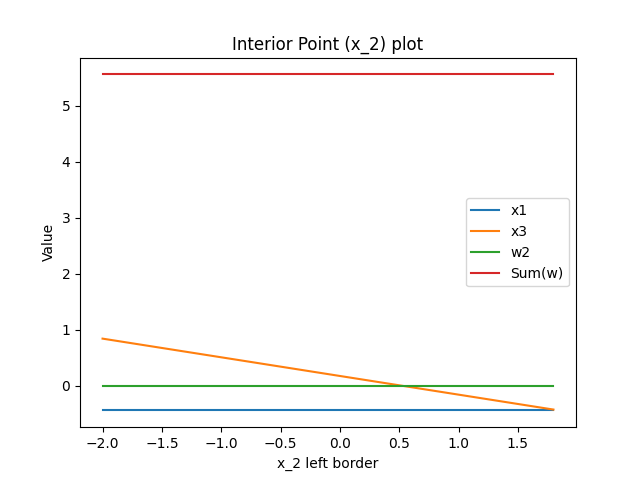
\includegraphics[width=0.5\textwidth]{interpoint(x_2).png}
	\caption{Зависимость от ограничений на $x_2$ при решении Interior-point-методом}
\end{figure} \\
Из графиков видно, что значение целевой функции не меняется, а координата $x_3$ зависит от ограничений на $x_2$ линейно.

\subsection{Ограничения на $x_3$}
Аналогично предыдущему пункту будем ограничивать координату $x_3$ интервалом ширины 0.2. Посмотрим на зависимость других координат решения, соответствующего масштабирующего коэффициента и целевой функции. Результаты представлены на графиках для 2 методов решения задачи ЛП. \\
\begin{figure}[h]
	\centering
	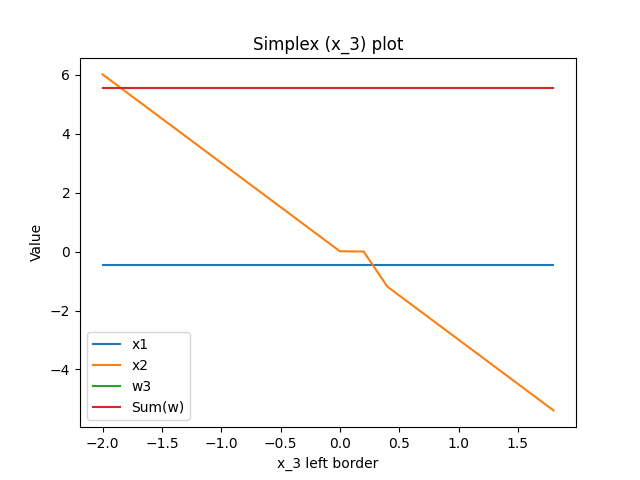
\includegraphics[width=0.5\textwidth]{simplex(x_3).png}
	\caption{Зависимость от ограничений на $x_3$ при решении Simplex-методом}
\end{figure}
\newpage
\begin{figure}[h]
	\centering
	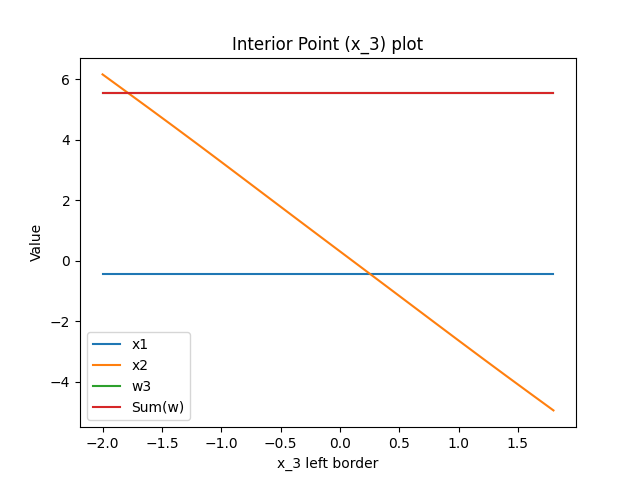
\includegraphics[width=0.5\textwidth]{interpoint(x_3).png}
	\caption{Зависимость от ограничений на $x_3$ при решении Interior-point-методом}
\end{figure}
Из графиков видно, что значение целевой функции не меняется, а координата $x_2$ зависит от ограничений на $x_3$ линейно.

\subsection{Ограничения на $x_2$ и $x_3$}
Теперь попробуем наложить ограничения на $x_2$ и $x_3$ одновременно. Иначе говоря, $x_2=[x_{2,3 \min}, x_{2,3 \min} + 0.2]$ и $x_3=[x_{2,3 \min}, x_{2,3 \min} + 0.2]$. Посмотрим, как будут зависеть координата $x_1$ и целевая функция.
\begin{figure}[h]
	\centering
	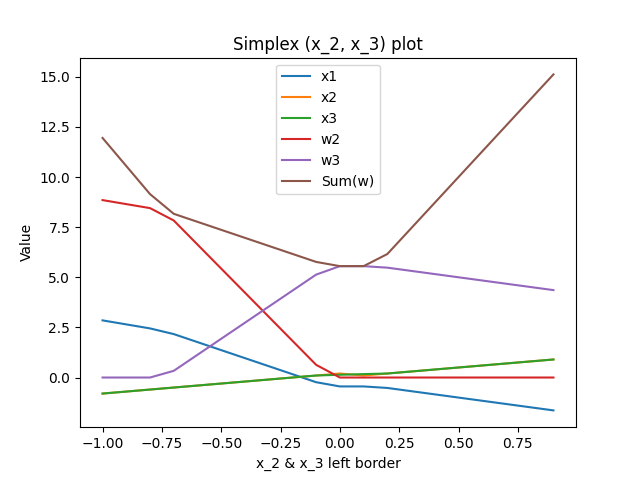
\includegraphics[width=0.5\textwidth]{simplex(x_2,x_3).png}
	\caption{Зависимость от ограничений на $x_2$ и $x_3$ при решении Simplex-методом}
\end{figure}
\newpage
\begin{figure}[h]
	\centering
	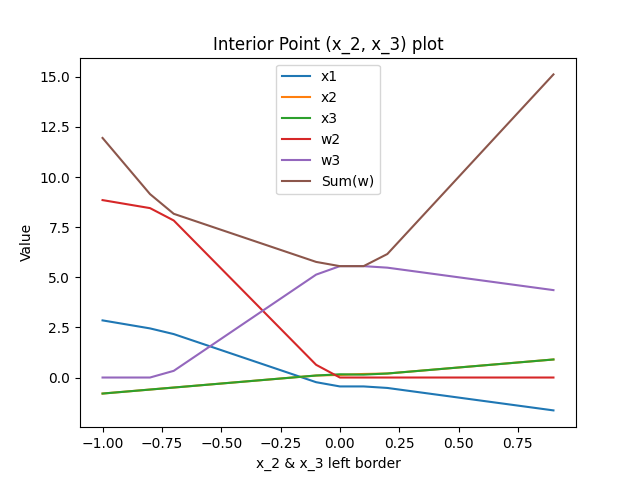
\includegraphics[width=0.5\textwidth]{interpoint(x_2,x_3).png}
	\caption{Зависимость от ограничений на $x_2$ и $x_3$ при решении Interior-point-методом}
\end{figure}
Из графиков видно, что минимум целевой функции 5.5555 достигается только тогда, когда $x_2$ и $x_3$ находятся примерно на отрезке $[0.1, 0.2]$.

\subsection{Анализ}
Таким образом, можно сделать вывод, что множество одинаково хороших решений задачи ЛП соответствует фиксированному значению $x_1=-0.4444$, и целой полосе возможных значений в осях $x_2(x_3)$ или $x_3(x_2)$.



\section{Приложение}
Код программы на Python лежит в данном репозитории: \\
\url{https://github.com/PinkOink/Interval_Analysis/tree/main/lab4}{}

Реализация функции tolsolvty на Python: \\
\url{https://github.com/MaximSmolskiy/tolsolvty}{}


\end{document}